\chapter{导数和微分}
本章将运用极限的方法给出导数和微分的概念,并对有关的基础知识,基本方法作简要介绍.

\section*{一、导数}

\section{平均变化率}

大家知道,若一辆汽车从上午8:30至10:00行驶了60千米,则在这段时间内汽车的平均速度为
\[\frac{\Delta S}{\Delta t}=\frac{60\text{千米}}{1.5\text{时}}=40\text{千米}/\text{时}\]

虽然汽车在行驶过程中的速度是不断变化的,但是这个平均速度表示了汽车在这段时间内,路程关于时间的平均变化率.

\noindent
\begin{minipage}{.48\textwidth}
    \CTEXindent
诸如像人口的出生率、导线的伸长系数、物体的膨胀系数等,都涉及了一个变量关于另一个变量的平均变化率.

对于函数$y=f(x)$,当自变量从$a$变化到$b$时,因变量的改变量$\Delta y=f(b)-f(a)$与自变量的改变量$\Delta x=b-a$的比,即
\[\frac{\Delta y}{\Delta x}=\frac{f(b)-f(a)}{b-a}\]
叫做$f(x)$从$a$到$b$之间的平均变化率.
\end{minipage}
\hfill
\begin{minipage}{.48\textwidth}
    \centering
\begin{tikzpicture}[>=stealth]
\draw[->](-.75,0)--(5,0)node[right]{$x$};
\draw[->](0,-1)--(0,3.5)node[left]{$y$};
\draw[domain=-.5:4.75, very thick, samples=100, smooth]plot(\x, {.15*(1*\x+.5)*(1*\x-2)*(1*\x-4)+1.5})node[left]{$y=f(x)$};
\tkzDefPoints{2.7/1.06/P, 4.25/1.9/Q}
\tkzDrawLines[add= .75  and .5](P,Q)
\tkzLabelPoints[above](P,Q)
\draw(4.25,1.06)--node[below]{$\Delta x$}(P)--(2.7,0)node[below]{$x_0$};
\draw(Q)--(4.25,0)node[below]{$x_0+\Delta x$};
\node [below left]{$O$};
\tkzDefPoints{2.7/0/A, 4.25/0/B, 4.25/1.06/C,0/0/O}
\tkzMarkRightAngles[size=.1](Q,C,P Q,B,A P,A,O)
\node at (4.25, 1.5)[right]{$\Delta y$};
\end{tikzpicture}
\captionof{figure}{}
\end{minipage}

如图12.1,设函数$y=f(x)$的图像是曲线$C$,对于曲线$C$上一点$P(x_0,y_0)$及点$P$邻近的任意一点$Q(x_0+\Delta x,y_0+\Delta y)$,不难得出割线的斜率就是函数$f(x)$从$x_0$到$x_0+\Delta x$之间的平均变化率,即    
\[K_{PQ}=\frac{\Delta y}{\Delta x}=\frac{f(x_0+\Delta x)-f(x_0)}{\Delta x}\]


\begin{example}
设一个质点在做非匀速运动中,位移$S$与时间$t$的函数关系是$S=4.9t^2+2t$,求此质点由时刻$t_0$到$t_0+\Delta t$的这段时间内运动的平均速度.
\end{example}

\begin{solution}
\[\begin{split}
    \Delta S&=[4.9(t_0+\Delta t)^2+2(t_0+\Delta t)]-(4.9t^2_0+2t_0)\\
&=9.8t_0\cdot \Delta t+2\Delta t+4.9(\Delta t)^2\\
\frac{\Delta S}{\Delta t}&=9.8t_0+2+4.9\Delta t
\end{split}\]
答:此质点由时刻$t_0$到$t_0+\Delta t$这段时间内运动的平均速度为$9.8t_0+2+4.9\Delta t$.
\end{solution}

\noindent
\begin{minipage}{.52\textwidth}
    \begin{example}
        如图12.2,设曲线$y=f(x)$与横轴$Ox$及直线$x=m$围成的面积为$S=g(m)=\frac{1}{2}m^3$, 
    \begin{enumerate}[(1)]
        \item 求函数$g(m)$从$m$到$m+\Delta m$之间的平均变化率;
        \item 当$|\Delta m|$的值愈来愈小,即$\Delta m\to 0$时,$g(m)$的平均变化率的极限是多少?
        \item 求$f(m)$.
    \end{enumerate}
    \end{example}
\end{minipage}\hfill
\begin{minipage}{.45\textwidth}
\centering
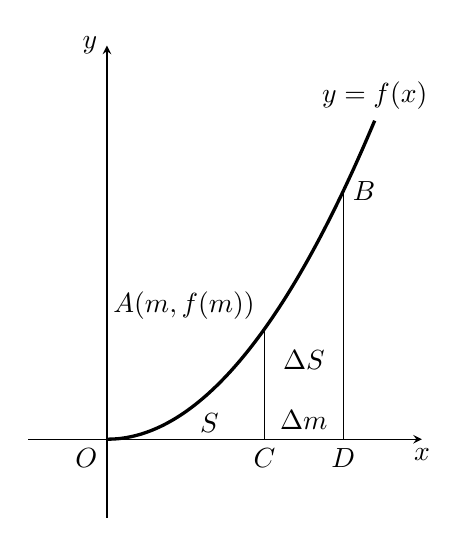
\begin{tikzpicture}[>=stealth, scale=2]
\draw[->](-.5,0)--(2,0)node[below]{$x$};    
\draw[->](0,-.5)--(0,2.5)node[left]{$y$};    
\draw[domain=0:1.7, very thick, smooth]plot(\x, {.7*\x^2})node[above]{$y=f(x)$};
\draw(1,0)node[below]{$C$}--(1,.7)node[above left]{$A(m,f(m))$};
\draw(1.5,0)node[below]{$D$}--(1.5,1.575)node[right]{$B$};
\node at (.65,.1){$S$};
\node at (1.25,.5){$\Delta S$};
\tkzDefPoints{0/0/O, 1.5/1.575/B, 1.5/0/D, 1/.7/A, 1/0/C}
\tkzMarkRightAngle[size=.1](A,C,O)
\node at (1.25,0)[above]{$\Delta m$};
\node [below left]{$O$};
\end{tikzpicture}
\captionof{figure}{}
\end{minipage}


\begin{solution}
\begin{enumerate}[(1)]
    \item 函数$g(m)$从$m$到$m+\Delta m$之间的平均变化率为
\[\begin{split}
\frac{\Delta S}{\Delta m}=\frac{g(m+\Delta m)-g(m)}{\Delta m}&=\frac{\frac{1}{2}(m+\Delta m)^3-\frac{1}{2}m^3}{\Delta m}\\
&=\frac{\frac{3}{2}m^2\cdot \Delta m+\frac{3}{2}m\cdot (\Delta m)^2+\frac{1}{2}(\Delta m)^3}{\Delta m}\\
&=\frac{3}{2}m^2+\frac{3}{2}m\cdot \Delta m+\frac{1}{2}(\Delta m)^2
\end{split}\]

\item $\Lim{\Delta m}{0}\frac{\Delta S}{\Delta m}=\Lim{\Delta m}{0}\left[\frac{3}{2}m^2+\frac{3}{2}m\cdot \Delta m+\frac{1}{2}(\Delta m)^2\right]=\frac{3}{2}m^2$

\item  当$|\Delta m|$充分小时,曲边梯形$ACDB$的面积$\Delta S$可用梯形$ACDB$的面积表示它的近似值,即$\Delta S\approx S_{\text{梯形}ACDB}$,因此$\frac{\Delta S}{\Delta m}\approx \text{梯形}ACDB$的中位线的长,

$\therefore\quad \Lim{\Delta m}{0}\frac{\Delta S}{\Delta m}=f(m)$,
即$f(m)=\frac{3}{2}m^2$.
\end{enumerate}
\end{solution}

\begin{ex}
\begin{enumerate}
    \item 已知函数$y=f(x)=x^2-x+2$的图象上有一动点$Q(x,y)$及定点$P(2,4)$.
\begin{enumerate}[(1)]
    \item 根据下表中$x_Q$的值,分别求出$f(x)$从2到$x_Q$之间的平均变化率;
\begin{center}
\begin{tabular}{c|ccccccc}
\hline
$x_Q$ & 4&3&2.5&2.1& 2.01& 2.001& 2.0001\\
\hline
$\Delta x$ \\
$\Delta y$ \\ [1.5ex]
$\frac{\Delta y}{\Delta x}$\\
\hline
\end{tabular}
\end{center}
\item 计算$\frac{f(2+\Delta x)-f(2)}{\Delta x}$
\item 计算$\Lim{\Delta x}{0}\frac{f(2+\Delta x)-f(2)}{\Delta x}$
\end{enumerate}

\item 对于12.1节中例12.1,计算$\Lim{\Delta t}{0}\frac{\Delta S}{\Delta t}$,并指出这个极限值的物理意义.
\item 已知$f(x)=\sqrt{25-x^2}$
\begin{enumerate}[(1)]
\item 计算$\frac{f(3+\Delta x)-f(3)}{\Delta x}$;
\item 计算$\Lim{\Delta x}{0}\frac{f(3+\Delta x)-f(3)}{\Delta x}$;
\item 试给出(2)中极限值的一种几何意义.
\end{enumerate}
\end{enumerate}
\end{ex}

\section{导数}
我们在研究函数$y=f(x)$的变量之间的关系时,不仅要
注意$f(x)$在$x_0$到$x_0+\Delta x$这一范围内的平均变化率,而且还要进一步研究当$\Delta x\to 0$时,$f(x)$在点$x=x_0$处的瞬时变化率. 例如,作非匀速直线运动的物体在某一时刻的瞬时速度;物体受热时,在某时刻温度的变化速度;导线在某时刻的电流强度;物质进行化学反应时,在某时刻的反应速度等.

设函数$y=f(x)$在点$x=x_0$及其附近有定义,$\Delta x$是自变量在点$x_0$的改变量,$\Delta y=f(x_0+\Delta x)-f(x_0)$是函数$f(x)$相应的改变量,若极限
\[\lim_{\Delta x\to 0}\frac{\Delta y}{\Delta x}=\lim_{\Delta x\to 0}\frac{f(x_0+\Delta x)-f(x_0)}{\Delta x}\]
存在,则称函数$f(x)$在点$x_0$处可导,且称此极限值为函数$f(x)$在点$x_0$的导数(即瞬时变化率,简称变化率),记作$f'(x_0)$或$y'\Big|_{x=x_0}$,于是
\[f'(x_0)=\lim_{\Delta x\to 0}\frac{\Delta y}{\Delta x}=\lim_{\Delta x\to 0}\frac{f(x_0+\Delta x)-f(x_0)}{\Delta x}\]

函数$f(x)$在点$x_0$处的导数$f'(x_0)$就是函数的平均变化率当$\Delta x\to 0$时的极限值,若极限值不存在,则称函数$f(x)$在点$x_0$处\textbf{不可导},即$f'(x_0)$不存在. 

若令$x=x_0+\Delta x$,代入上式,得
\[f'(x_0)=\lim_{x\to x_0}\frac{f(x)-f(x_0)}{x- x_0}\]
这是求$f'(x_0)$常用的另一种表达式.


\begin{example}
    已知$f(x)=\sqrt{x}$,求$f'(1)$, $f'(2)$
\end{example}

\begin{solution}
\[\begin{split}
f'(1)&=\Lim{x}{1}\frac{f(x)-f(1)}{x-1}=\Lim{x}{1}\frac{\sqrt{x}-1}{x-1}\\
&=\Lim{x}{1}\frac{\sqrt{x}-1}{(\sqrt{x}-1)(\sqrt{x}+1)}=\Lim{x}{1}\frac{1}{\sqrt{x}+1}=\frac{1}{2}\\
f'(2)&=\Lim{\Delta x}{0}\frac{f(2+\Delta x)-f(2)}{\Delta x}=\Lim{\Delta x}{0}\frac{\sqrt{2+\Delta x}-\sqrt{2}}{\Delta x}\\
&=\Lim{\Delta x}{0}\frac{\Delta x}{\Delta x\left(\sqrt{2+\Delta x}+\sqrt{2}\right)}\\
&=\Lim{\Delta x}{0}\frac{1}{\sqrt{2+\Delta x}+\sqrt{2}}=\frac{1}{2\sqrt{2}}
\end{split}\]
$\therefore\quad f'(1)=\frac{1}{2},\quad f'(2)=\frac{\sqrt{2}}{4}$
\end{solution}

\begin{example}
已知$f(x)=|x|$,求$f'(-1)$,$f'(0)$
\end{example}

\begin{solution}
\[\begin{split}
    f'(-1)&=\Lim{x}{-1}\frac{f(x)-f(-1)}{x-(-1)}= \Lim{x}{-1}\frac{|x|-1}{x+1}\\
    &=\Lim{x}{-1}\frac{-(x+1)}{x+1}=\Lim{x}{-1}(-1)=-1
\end{split} \]
$\therefore\quad f'(-1)=-1$

当$x\to 0$时,$\frac{\Delta y}{\Delta x}=\frac{|\Delta x|}{\Delta x}$

$\because\quad $当$\Delta x>0$时,$\frac{|\Delta x|}{\Delta x}=1$;当$\Delta x<0$时,$\frac{|\Delta x|}{\Delta x}=-1$

$\therefore\quad \Lim{\Delta x}{0}\frac{\Delta y}{\Delta x}=\Lim{\Delta x}{0}\frac{|\Delta x|}{\Delta x}$不存在,即$f(x)=|x|$在$x=0$时没有导数,$f'(0)$不存在.
\end{solution}

\begin{ex}
\begin{enumerate}
    \item 求$f'(2)$
\begin{multicols}{2}
\begin{enumerate}[(1)]
    \item $f(x)=x^3$
    \item $f(x)=\frac{1}{x}$
    \item $f(x)=-2x^2+3x+1$
\end{enumerate}
\end{multicols}
    \item 已知$f(x)=\sin x$,求:$f'\left(\frac{\pi}{6}\right)$、$f'\left(\frac{\pi}{2}\right)$
\end{enumerate}
\end{ex}

\section{导数的几何意义}
在12.1节中我们已经知道,若点$Q(x_0+\Delta x,y_0+\Delta y)$、$P(x_0,y_0)$分别是函数$y=f(x)$的图象上的两点,则割线的斜率为
\[K_{PQ}=\frac{\Delta y}{\Delta x}=\frac{f(x_0+\Delta x)-f(x_0)}{\Delta x}\]

若函数$f(x)$在点$x_0$处可导,则
\[f'(x_0)=\lim_{\Delta x\to 0}\frac{\Delta y}{\Delta x}=\lim_{\Delta x\to 0}\frac{f(x_0+\Delta x)-f(x_0)}{\Delta x}\]

当$\Delta x\to 0$时,如图12.3,点$Q(x_0+\Delta x,y_0+\Delta y)$沿着函数
$y=f(x)$的图象无限地趋近于$P(x_0,y_0)$点,这时割线$PQ$绕着点$P$转动,它的极限位置是函数$y=f(x)$的图象在点$P$处的切线. 因此,
\[K_{PT}=\lim_{Q\to P}K_{PQ}=\lim_{\Delta x\to 0}\frac{\Delta y}{\Delta x}=f'(x_0)\]

\begin{figure}[htp]
    \centering
\begin{tikzpicture}[>=stealth, scale=1.5]
\draw[->](-.75,0)--(5,0)node[right]{$x$};
\draw[->](0,-1)--(0,3.5)node[left]{$y$};
\draw[domain=-.5:4.75, very thick, samples=100, smooth]plot(\x, {.15*(1*\x+.5)*(1*\x-2)*(1*\x-4)+1.5})node[left]{$y=f(x)$};
\tkzDefPoints{3.5/1.05/P, 4.25/1.9/Q}
\tkzDrawLines[add= 2.5  and .75](P,Q)
\tkzLabelPoints[above](P)
\tkzLabelPoints[above left](Q)
\draw(4.25,1.06)--node[below]{$\Delta x$}(P)--(3.5,0)node[below]{$x_0$};
\draw(Q)--(4.25,0)node[below]{$x_0+\Delta x$};
\node [below left]{$O$};
\tkzDefPoints{3.5/0/A, 4.25/0/B, 4.25/1.05/S,0/0/O}
\tkzMarkRightAngles[size=.1](Q,S,P Q,B,A P,A,O)
\tkzLabelPoints[right](S)

\tkzDefPoints{4.25/1.7/Q1, 4.25/1.6/Q2, 4.25/1.5/Q3, 4.25/1.4/Q4}

\foreach \x in {1,2,3}
{
    \tkzDrawLines[add= 3  and .75](P,Q\x)
}

\tkzDrawLines[add= 4.5  and .75, very thick](P,Q4)
\node at (4.75,1.65)[right]{$T$};

\end{tikzpicture}
    \caption{}
\end{figure}

综上所述,函数$y=f(x)$在
点$x_0$处的导数$f'(x_0)$的几何意
义是曲线$y=f(x)$在点$(x_0,f(x_0))$处的切线的斜率.

\begin{example}
求与曲线$y=x^3$相切于点$A(-1,-1)$的切线方程,并作图.
\end{example}

\noindent
\begin{minipage}{.55\textwidth}
    \begin{analyze}
        欲求以点$A(-1,-1)$为切点的切线方程,只需求出切线的斜率,而$K_{\text{切}}=f'(-1)$.
    \end{analyze}
    
    \begin{solution}
\[\begin{split}
    K_{\text{切}}=f'(-1)&=\lim_{x\to -1}\frac{f(x)-f(-1)}{x-(-1)}\\
    &=\lim_{x\to -1}\frac{x^3+1}{x+1}\\
    &=\lim_{x\to -1}(x^2-x+1)=3
\end{split}\]
\[\begin{split}
    y-(-1)&=3[x-(-1)]\\
    y+1&=3x+3
\end{split}\]
$\therefore\quad y=3x+2$为所求的切线方程. 

作图如图12.4.    
\end{solution}
\end{minipage}
\begin{minipage}{.4\textwidth}
\centering
\begin{tikzpicture}[>=stealth, scale=.5]
\draw[->](-4,0)--(5,0)node[below]{$x$};    
\draw[->](0,-3)--(0,10)node[left]{$y$};
\draw[domain=-1.3:2.1, smooth, very thick, samples=100]plot(\x, {\x^3});
\node[below right]{$O$};
\tkzDefPoints{-1/-1/A, 2/8./B}
\tkzDrawLines[](A,B)
\node at (A)[left] {$A(-1,-1)$};
\node at (B)[right] {$B(2,8)$};
\tkzDrawPoints(A,B)
\node at (-.25,1.25)[left]{$y=3x+2$};
\node at (1.5,3.375)[right]{$y=x^3$};
\end{tikzpicture}
\captionof{figure}{}
\end{minipage}
    
\begin{example}
求过曲线$y^2=2px\; (y\ge 0)$上一点$P(x_0,y_0)$的切线方程.
\end{example}

\begin{solution}
$y=\sqrt{2px}\quad (y\ge 0,\; x\ge 0)$
\[\begin{split}
    y^{\prime}\Big|_{x=x_{0}}=\lim_{x\to x_{0}}\frac{\sqrt{2px}-\sqrt{2px_{0}}}{x-x_{0}}&=\lim_{x\to x_{0}}\frac{\sqrt{2p}(\sqrt{x}-\sqrt{x_{0}})}{(\sqrt{x}-\sqrt{x_{0}})(\sqrt{x}+\sqrt{x_{0}})}\\
    &=\lim_{x\to x_{0}}\frac{\sqrt{2p}}{\sqrt{x}+\sqrt{x_{0}}}=\sqrt{\frac{p}{2x_{0}}}\\
\end{split}\]
以$P(x_0,y_0)$为切点做切线方程为
\[\begin{split}
    y-y_0&=\sqrt{\frac{p}{2x_0}}(x-x_0)\\
    y-\sqrt{2px_0}&=\sqrt{\frac{p}{2x_0}}x-\sqrt{\frac{px_0}{2}}\\
y&=\sqrt{\frac p{2x_{0}}}x+\sqrt{\frac{px_{0}}2}=\frac{p}{\sqrt{2px_{0}}}(x+x_{0})
\end{split}\]
$\therefore\quad y_{0}y= p( x+ x_{0})$为所求切线方程.
\end{solution}

\begin{ex}
\begin{enumerate}
    \item 已知曲线$y=x^2-x$,分别求出在下列点处的切线方程:
\begin{multicols}{2}
\begin{enumerate}[(1)]
    \item $A(1,0)$
    \item $B(0,0)$
\end{enumerate}
\end{multicols}
    \item 求曲线$y=6x^{-1}$在点$A(3,2)$处的切线方程.
    \item 若函数$f(x)$在点$x_0$处及其附近可导,当$|\Delta x|$很小时,$\Delta y\approx$\blank .
\end{enumerate}
\end{ex}

\section{函数可导与连续的关系}
由12.2节中的例12.4可知,函数$f(x)=|x|$在$x=0$时连续,但$f'(0)$不存在.因此.若函数$f(x)$在点$x_0$处连续,函数$f(x)$在该点不一定可导. 反过来,若函数$f(x)$在点$x_0$处可导,则可以证明函数$f(x)$在该点一定连续. 事实上,欲证$f(x)$在点$x_0$处连续,只需证
$\Lim{x}{x_0}f(x)=f(x_0)$.

\[\begin{split}
\because\quad \Lim{x}{x_0}f(x)&=\Lim{x}{x_0}[f(x)-f(x_0)+f(x_0)]=\Lim{x}{x_0}[f(x)-f(x_0)]+f(x_0)\\
&=\Lim{x}{x_0}\left[\frac{f(x)-f(x_0)}{x-x_0}\cdot (x-x_0)\right]+f(x_0)\\
&=\Lim{x}{x_0} \frac{f(x)-f(x_0)}{x-x_0}  \cdot \Lim{x}{x_0}(x-x_0)+f(x_0)\\
&=f'(x_0)\cdot 0+f(x_0) =f(x_0)
\end{split}\]

$\therefore\quad \Lim{x}{x_0}f(x)=f(x_0)$即$f(x)$在点$x_0$处连续.

\begin{thm}{定理}
    若函数$f(x)$在点$x_0$处可导,则函数$f(x)$在点$x_0$处也连续.
\end{thm}

\begin{example}
    已知 函数$f(x)=|x^2-1|$
\begin{enumerate}[(1)]
\item 函数在$x_1=-1,\; x_2=0,\; x_3=-1$是否连续?
\item 函数在$x_1=-1,\; x_2=0,\; x_3=-1$是否可导?
\end{enumerate}
\end{example}

\begin{solution}
\[f(x)=|x^2-1|=\begin{cases}
    x^2-1,& x\le -1\; \text{或}\; x\ge 1\\
    1-x^2,& -1\le x\le 1
\end{cases}\]
\begin{enumerate}[(1)]
    \item $\because\quad \Lim{x}{0}f(x)=\Lim{x}{0}(1-x^2)=1=f(0)$

    $\therefore\quad f(x)$在$x=0$处连续.

$\because\quad \Lim{x}{1^+}f(x)=\Lim{x}{1^+}(x^2-1)=0,\;  \Lim{x}{1^-}f(x)=\Lim{x}{1^-}(1-x^2)=0,\; f(1)=0$

$\therefore\quad f(x)$在$x=1$处连续. 同理可证$f(x)$在$x=-1$处连续.

\item $\because\quad \Lim{x}{0}\frac{f(x)-f(0)}{x}=\Lim{x}{0}\frac{1-x^2-1}{x}=\Lim{x}{0}(-x)=0$

$\therefore\quad f'(0)$存在,且$f'(0)=0$
\[\begin{split}
  \because\quad  \Lim{x}{1^+}\frac{f(x)-f(1)}{x-1}&= \Lim{x}{1^+}\frac{x^2-1}{x-1}= \Lim{x}{1^+}(x+1)=2\\
  \Lim{x}{1^-}\frac{f(x)-f(1)}{x-1}&=\Lim{x}{1^-}\frac{1-x^2}{x-1}=-\Lim{x}{1^-}(x+1)=-2
\end{split}\]
$\therefore\quad f(x)$在$x=1$处不可导. 同理可证,$f(x)$在$x=-1$处也不可导.
\end{enumerate}
\end{solution}

\begin{ex}
\begin{enumerate}
    \item 作函数$y=|x^2-x|$的图象,并说明它在哪个点不可导.
    \item 已知函数$f(x)=\begin{cases}
        x\sin\frac{1}{x},& x\ne 0\\
        0,& x=0
    \end{cases}$

    试说明此函数$f(x)$在点$x=0$处是否可导及连续.
\end{enumerate}
\end{ex}

\section*{习题一}
\begin{center}
    \bfseries A
\end{center}

\begin{enumerate}
    \item 分别求下列函数的平均变化率$\frac{\Delta y}{\Delta x}$:
\begin{enumerate}[(1)]
    \item $y=-2x^3+x^2-1$,当$x=1$, $\Delta x=0.1$时;
    \item $y=\frac{x}{3}$,当$x=2$, $\Delta x=0.01$时;
    \item $y=\sqrt{2x}$,当$x=4$, $\Delta x=0.001$时.
\end{enumerate}
    ((2)、(3)题精确到0.001)
    \item     根据导数定义,求下列函数在给定点的导数:
\begin{multicols}{2}
\begin{enumerate}[(1)]
    \item $y=-2x^3+x^2-1$,求$f'(1)$;
    \item $y=\frac{3}{x}$,求$f'(2)$;
    \item $y=\sqrt{2x}$,求$f'(4)$.
\end{enumerate}
\end{multicols}
    \item    一质点做直线运动,它所经过的路程和时间的关系是$s=3t^2+2t+1$,求$t=2$时的瞬时速度.
    \item    求曲线$y=x^3$在点$A(2,8)$处的切线方程.
\end{enumerate}

\begin{center}
    \bfseries B
\end{center}

\begin{enumerate}\setcounter{enumi}{4}
    \item 已知$f(x)=\begin{cases}
        x^2\sin\frac{1}{x},& x\ne 0\\
        0,& x=0
    \end{cases}$,求$f'(0)$.
\item 函数$y=|\sin x|$在$x=0$处是否存在导数?并说明你的理由.
\item 已知$f(x)=\begin{cases}
    2x^2,& x\le 1\\
-2x^2+8x-4,& x\ge 1
\end{cases}$
,求$f'(1)$
\item 设$f(x)$在点$x=1$处的导数为$f'(1)$,计算
\begin{multicols}{2}
\begin{enumerate}[(1)]
    \item $\Lim{h}{0}\frac{f(1+3h)-f(1)}{h}$
    \item $\Lim{h}{0}\frac{f(1+h)-f(1-h)}{2h}$
\end{enumerate}
\end{multicols}
\end{enumerate}

\section*{二、函数的导数}

\section{函数的导数}

我们已经学了函数$f(x)$在点$x_0$处的导数,例如$f(x)=\frac{1}{x}$在点$x_0$处的导数为:
\[\begin{split}
f'(x_0)&=\Lim{h}{0}\frac{f(x_0+h)-f(x_0)}{h}=\Lim{h}{0}\frac{\frac{1}{x_0+h}-\frac{1}{x_0}}{h}\\
&=\Lim{h}{0}\frac{x_0-(x_0+h)}{hx_0(x_0+h)}=\Lim{h}{0}\frac{-1}{x_0(x_0+h)}=-\frac{1}{x^2_0}
\end{split}\]
即:$f'(x_0)=-\frac{1}{x^2_0}$

如果$x_0\in (0,+\infty)$,不难看出,对于开区间$(0,+\infty)$内每一个确定的值$x_0$,都有唯一确定的值$f'(x_0)$与其相对应,这样,在开区间$(0,+\infty)$内,利用求导的方法又得到了一个新
的函数$f'(x)=-\frac{1}{x^2}$.

一般地,若函数$f(x)$在开区间$(a,b)$内每一点$x$处都可导,即.
\[f'(x)=\Lim{h}{0}\frac{f(x+h)-f(x)}{h}\qquad x\in(a,b)\]
则由此对应法则确定的函数$f'(x)$叫做函数$f(x)$的导函数(简称$f(x)$的导数)。这时又称$f(x)$在开区间$(a,b)$内可导.

下面根据函数的导数定义,求几种最常见的函数的导数.
\begin{enumerate}
    \item $f(x)=c$($c$为常数)的导数.

    $\because\quad f'(x)=\Lim{h}{0}\frac{f(x+h)-f(x)}{h}=\Lim{h}{0}\frac{c-c}{h}=0$

$\therefore\quad    f'(x)=c'=0$($c$为常数).
    \item $f(x)=x^n$($n$为自然数)的导数.
\[\begin{split}
    \because\quad f'(x)&=\Lim{h}{0}\frac{f(x+h)-f(x)}{h}=\Lim{h}{0}\frac{(x+h)^n-x^n}{h}\\
&=\Lim{h}{0}\left({\rm C}^1_n x^{n-1}+{\rm C}^2_nx^{n-2}\cdot h+\cdots+{\rm C}^k_nx^{n-k}\cdot h^{k-1}+\cdots +h^{n-1}\right)\\
&={\rm C}^1_nx^{n-1}=nx^{n-1}
\end{split}\]
$\therefore\quad f'(x)=(x^n)'=nx^{x-1}$($n$为自然数).
    \item $f(x)=\sin x$的导数.
    \[\begin{split}
        \because\quad f'(x)&=\Lim{h}{0}\frac{f(x+h)-f(x)}{h}=\Lim{h}{0}\frac{\sin (x+h)-\sin x}{h}\\
    &=\Lim{h}{0}\frac{2\cos \left(x+\frac{h}{2}\right)\sin \frac{h}{2}}{h}\\
    &=\Lim{h}{0}\cos \left(x+\frac{h}{2}\right)\cdot \Lim{\tfrac{h}{2}}{0}\frac{\sin\frac{h}{2}}{\frac{h}{2}}=\cos x
    \end{split}\]
    $\therefore\quad f'(x)=(\sin x)'=\cos x$.

\item $f(x)=\cos x$的导数.
\[\begin{split}
    \because\quad f'(x)&=\Lim{h}{0}\frac{f(x+h)-f(x)}{h}=\Lim{h}{0}\frac{\cos (x+h)-\cos x}{h}\\
&=\Lim{h}{0}\frac{-2\sin \left(x+\frac{h}{2}\right)\sin \frac{h}{2}}{h}\\
&=-\Lim{h}{0}\sin \left(x+\frac{h}{2}\right)\cdot \Lim{\tfrac{h}{2}}{0}\frac{\sin\frac{h}{2}}{\frac{h}{2}}=-\sin x
\end{split}\]
$\therefore\quad f'(x)=(\cos x)'=-\sin x$.

\item $f(x)=\ln x$的导数.
\[\begin{split}
    \because\quad f'(x)&=\Lim{h}{0}\frac{f(x+h)-f(x)}{h}=\Lim{h}{0}\frac{\ln (x+h)-\ln x}{h}\\
&=\Lim{h}{0}\frac{1}{h}\ln\left(1+\frac{h}{x}\right)=\Lim{h}{0}\left[\frac{1}{x}\cdot \frac{x}{h}\ln\left(1+\frac{1}{\frac{x}{h}}\right)\right]\\
&=\frac{1}{x}\lim_{\tfrac{x}{h}\to \infty}\ln\left(1+\frac{1}{\frac{x}{n}}\right)^{\tfrac{x}{h}}=\frac{1}{x}\ln\left[\lim_{\tfrac{x}{h}\to\infty}\left(1+\frac{1}{\frac{x}{h}}\right)^{\tfrac{x}{h}}\right]\\
&=\frac{1}{x}\ln e=\frac{1}{x}
\end{split}\]
$\therefore\quad f'(x)=(\ln x)'=\frac{1}{x},\quad (x>0)$.
\end{enumerate}

综上所述,目前我们得到几种最常见的函数的导数为(今后可当公式用):
\begin{thm}{}
   \begin{enumerate}
\item $c'=0$($c$为常数).
\item $(x^n)'=nx^{n-1}$($n$为自然数).
\item $(\sin x)'=\cos x$.
\item $(\cos x)'=-\sin x$.
\item $(\ln x)'=\frac{1}{x}$
\end{enumerate}     
\end{thm}

\begin{ex}
\begin{enumerate}
    \item 求下列函数的导数:
\begin{multicols}{2}
\begin{enumerate}[(1)]
\item $f(x)=x^{10}$;
\item $f(x)=x^{99}$;
\item $f(x)=\cos x$;
\item $f(x)=\ln x$.
\end{enumerate}
\end{multicols}
    \item 根据函数的导数定义,求下列函数的导数.
\begin{multicols}{2}
\begin{enumerate}[(1)]
\item $f(x)=3x^4+2x^3$;
\item $f(x)=\frac{1}{x^2}$;
\item $f(x)=\sqrt{x}$;
\item $f(x)=\sin3x$;
\item $f(x)=\cos(-2x)$.
\end{enumerate}
\end{multicols}
\end{enumerate}
\end{ex}

\section{函数的和、差、积、商的导数}
如同研究函数极限的四则运算一样,下面研究函数的四则运算的导数.

已知函数$f(x)$、$g(x)$的导数分别为$f'(x)$、$g'(x)$











\begin{example}
    
\end{example}

\begin{solution}
    
\end{solution}



\begin{example}
    
\end{example}

\begin{solution}
    
\end{solution}


\begin{example}
    
\end{example}

\begin{solution}
    
\end{solution}


\begin{example}
    
\end{example}

\begin{solution}
    
\end{solution}


\begin{example}
    
\end{example}

\begin{solution}
    
\end{solution}




